\chapter{Methods and Implementation}
\setcounter{chapter}{3}
\section{\alg}

Summarizing the key points made in chapter \ref{background}, generalization is in large part a function of the causal robustness of the features that the model learns. The problem of achieving generalization, then, boils down to imposing constraints to the optimization procedure such that the model ignores non-causal patterns.

Directly discriminating between causal and non-causal patterns is, however, somewhat intractable. For one, the patterns that neural networks learn are often difficult to identify, and even more difficult to understand semantically. Secondly, even if these patterns could be understood, establishing causality necessitates a complete understanding of the same problem the model is trying to learn. Thus, if it was at all possible to establish causality, one might as well use the knowledge required to do so to design a classifier using conventional image-analysis. 

Though establishing what is causal is difficult, establishing what \textit{isn't} causal is not all that complicated. To give a concrete example, consider once again classifying images of cows and camels. Associating the cow class with grass is obviously non-causal, and does not hold if the cow for instance is modifyed such that the same cow now is instead pictured on mars. Neither will associating the cow class with the colour of its coat, as this will not hold if the model is for instance used to classify a black-and-white version of the same image. The more of these non-causal changes to the input data- from this point on referred to as perturbations - are excluded from the search, the more likely the model is to learn the patterns that are actually causal. After all, a pattern can for all intents and purposes be considered causal when it holds when subjected to all non-causal perturbations. 

Thus, though rewarding causal behaviour is intractable, punishing non-causal behaviour is not. All that is required to do so is to be able to apply perturbations that highlight the non-causal reasoning the model employs, quantify the model's sensitivity to these perturbations, then minimize this quantity through optimization. The resulting model will then have learned invariance to whatever causally irrelevant confounding variable that the perturbation defines. This property of being invariant to perturbations will be referred to as the consistency of the model. 

Thus, consistency is in effect a surrogate for generalizability; if a model is consistent, it is invariant to non-causal patterns, and if it is invariant to non-causal patterns, it necessarily employs causal patterns. Optimizing for consistency can as a result mitigate both shortcut-learning and underspecification, subject only to the span of the space of perturbations and how well inconsistent behaviour can be quantified. For instance, if the perturbations affect the image such that certain shortcuts are broken, these shortcuts are less likely to be learned. A similar argument can be made for underspecification: if multiple predictors are risk equivalent but nevertheless encode conflicting inductive biases, probing the respective predictors through various perturbations specifically targeting these inductive biases can reveal which are generalizable and which are not.

Naturally, this all presupposes that there is some model that can output all possible perturbations. This is of course not the case; it would obviously not be a simple matter to send cows to mars or camels to the moon to induce invariance to backgrounds in the aforementioned example. However, even if the model is subjected only to a few perturbations, this nevertheless increases the likelihood of achieving generalisability by virtue of the fact that it limits the search space to predictors that exhibit invariance to these perturbations. Thus, though generalizability is by no means guaranteed by this approach, defining a certain set of perturbations for which the model should exhibit invariance to is nevertheless likely to nevertheless improve out-of-distribution performance. 

Additionally, this approach requires that there is some way to quantify the inconsistency across these perturbations. 

\subsection{Consistency Loss}    
    In order to bias the pipeline towards inferring causally reasonable inductive biases, the model needs to be able to learn to be robust to distributional shifts that are known not to affect the causal structure of the problem. These types of distributional shift, from this point referred to as perturbations, should not affect the predictions of the model beyond what one would expect. I.e, if an image is rotated, the only change one should expect in the segmentation is a corresponding rotation. If an image is globally distorted in some way, the segmentation should exhibit the corresponding distortion. If an image is exposed to low-amplitude additive noise, the segmentation should not really be affected at all, and so on. This property will be referred to as the consistency of the model. By definition, the model needs to be consistent in order to have a chance at being generalizable. Consequently, one can optimise for and maximise consistency as a partial surrogate for generalizability. Expressed as a minimisation problem, this corresponds to minimising inconsistency. A loss function that can describe inconsistent behaviour is therefore necessary. In other words, the loss function needs to be able to express numerically the discrepancy between the expected change in the segmentation and the actual change in the segmentation when subjected to some perturbation. Formally, this can be expressed as follows:

	Let \(Y:=\{y,\hat{y}:=f(x)\}\) be the set consisting of the segmentation labels (masks) and predictions for the unperturbed samples. Let \(\epsilon(\cdot)\) be some perturbation function. Then, let \(A:=\{a:=\epsilon(y),\hat{a}:=f(\epsilon(x))\}\) be the set consisting of segmentation predictions and masks when the input is subjected to this perturbation. Inconsistency can then be defined by:
    \begin{equation}
		L_c = \frac{1}{\sum\{y \cup a \}} \sum \{y\ominus\hat{y}\ominus a\ominus\hat{a}\}
	\end{equation}
    Where \(\ominus \) denotes the symmetric difference. 
	This corresponds to counting the number of pixels that change after the input is subjected to a perturbation - \(\hat{a}\ominus \hat{y}\), but discounting those we expect to change, \(a\ominus y\). 
	This loss is minimised not only if the predictions are both correct and consistent with one another, but also if the predictions are both incorrect, so long as whatever change that occurs is consistent with the expected change. This is illustrated in Figure \ref{loss_fn}
    \begin{figure}[h]
        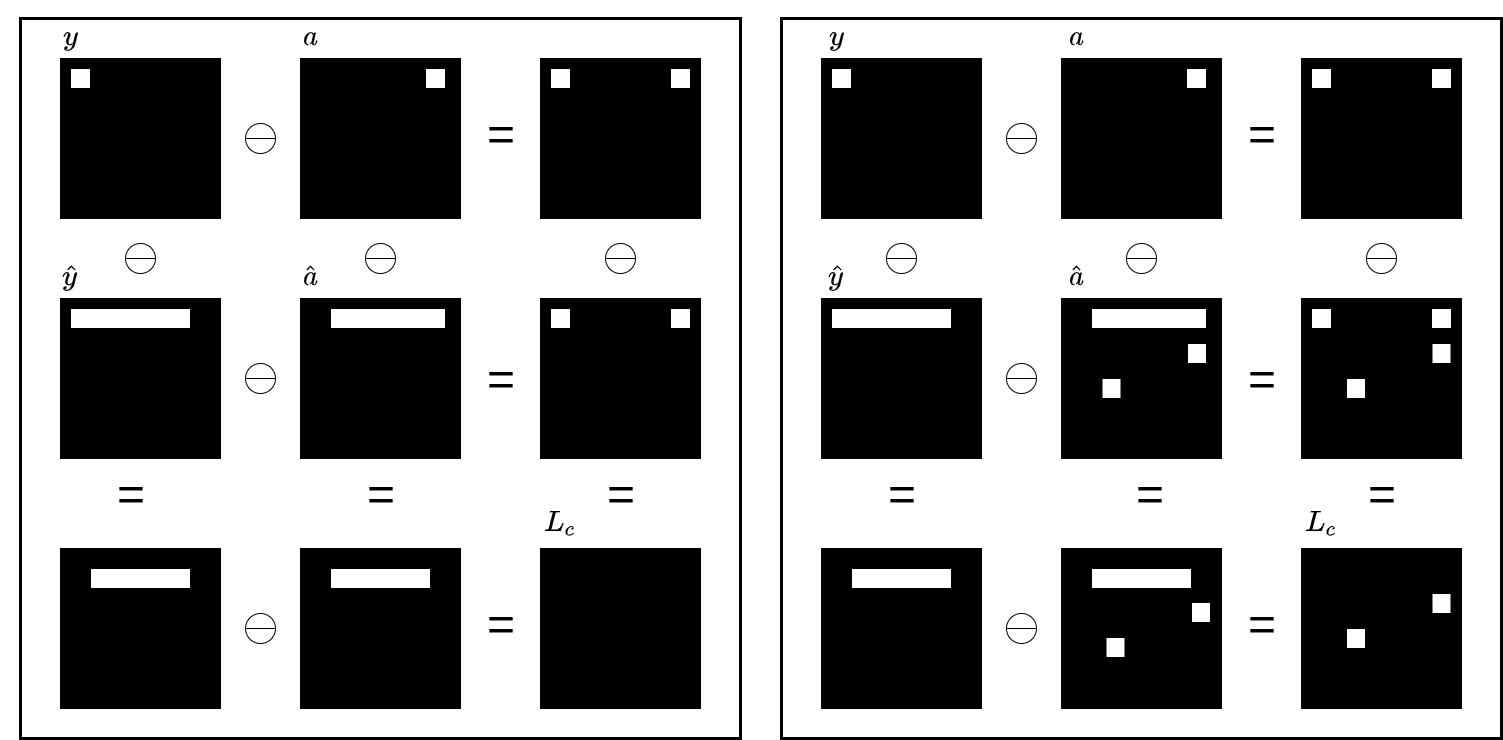
\includegraphics[width=\linewidth]{illustrations/loss_visualisation.drawio.png}
        \caption{Visualisation of consistency loss sets, where white is a positive prediction. Note that loss is zero regardless of prediction correctness so long as it changes in the expected manner. Note also that the symmetric difference operators are associative}
        \label{loss_fn}
    \end{figure}  

    The reasoning behind this is that consistent behaviour should be rewarded even if the model has not quite learned how to perform to an adequate standard, as this is preferable to merely learning to perform well without any regard for consistency and by extension causality.  To illustrate, consider once more the example from chapter \ref{background}, namely the problem of acheiving generalisation from narrow-band to white-light imaging datasets and vice versa. Assume that the perturbation function simply maps between the respective lighting modalities. In this case, the loss will reward the model if it predicts identical segmentations regardless of lighting conditions, even if the predictions are incorrect. The model will nevertheless be trying to leverage features which are invariant to lighting, and consequently be more generalizable than a pipeline wherein the model is permitted to be leverage lighting-dependent features.
        
    Note, however, that the loss does not presuppose what transformation has occurred. In Figure \ref{loss_fn}, for instance, the change induced by the perturbation may correspond to simply moving the polyp in the image (and replacing the empty space with a believable background), or it may correspond to a rotation by 90 degrees. How this should affect the segmentations is up to interpreation - one can argue that a rotation should rotate the incorrect predictions as well, or one can argue that it should only rotate the correct component of the prediction. For simplicity, consistency loss adheres to the latter argument, though it should be noted that designing loss functions that account for the former case is also an interesting direction to pursue. 
	
	Moreover, using this loss in isolation is not really practical. For one, the model will have no way of knowing what the actual intent behind it is, and moreover the model will most likely learn the simplest possible interpretation of consistency and simply predict the same segmentation every time, with the only difference being whatever it learns constitutes expected change. This constitutes fairly broad local minima, and there would naturally be a significant number of risk-equivalent predictors, which of course in accordance with the analysis in \ref{background} constitutes generalisation failure on its own. Thus, it has to be combined with a task-specific loss, which for the polyp-segmentation task could be Dice-loss, Jaccard-Loss, binary cross entropy, etc. 
	
	Naturally, jointly optimizing for these two often conflicting objectives - overall task performance vs consistency - is not straight forward. The naive approach would be to simply add the task-loss and the naked consistency:
    \begin{equation}
		L = L_{task} + L_c
	\end{equation}
	This, however, leads to unstable behaviour and often inhibits convergence, since the consistency term quickly starts gaining precedence if the segmentation task is difficult (see appendix). Consequently, adaptive weighing is required. To avoid getting stuck in broad local minima early, the training should in the early stages be biased towards acheiving semi-decent segmentation performance. Later on, when segmentation performance is starting to become reasonably high, the pipeline should shift towards trying to optimize for consistency. This can be acheived by weighing each term according to a desired performance metric, for instance intersection over union (IoU):
	\begin{equation}
		L = (1-IoU)\times L_{task} + IoU \times L_c
	\end{equation}
	If Jaccard loss is used, this is also equivalent to:
	\begin{equation}
		L = {L_{jac}}^2 + (1-L_{jac})\times L_c
	\end{equation}
	
  	\subsection{Model of natural variation}
  	In order to account for any natural variation one may expect to find in deployment, it is necessary to construct a model which can parameterize the variability that is encountered. This model of natual variation, or MNV, can then be leveraged in conjunction with consistency loss to facilitate the learning of features that are robust to the types of variation the MNV defines. Naturally, there is no way of knowing the full extent of all the types of variability one may find in the wild, but it may nonetheless be sufficient to model some subset thereof. This, naturally, requires some knowledge of the domain from which the dataset is collected. Similarly to how adding rotational augmentations is a bad idea for classification of hand-written numbers, certain transformations may or may not be suitable for use within a MNV.
  		
  	In the case of polyp-segmentation, it is clear that it is necessary to account for variability in for instance lighting, image-resolution, polyp-size, polyp-shape, polyp-location, camera-quality, color-shifts, blurs, optical distortions, and affine transformations. Thus, a model is required that can (more or less) parametrize this variability. Broadly speaking, these transformations can be categorized as follows:
    \begin{itemize}
        \item Pixel-wise variability, which affect only the image, i.e color-shifts, brightness shifts, contrast-shifts, lighting, blurs etc
        \item Geometric variability, which affect both the image and the segmentation mask by some parametrizable quantity, i.e affine transforms and distortions
        \item Manifold variablity, which affects both the image and the segmentation mask depending on a learned model of the distribution,  i.e the size, shape and location of polyps
    \end{itemize}
    Pixel-wise variability and geometric variability can be modeled fairly trivially through the use of the same transformations typically used in conventional data-augmentation. Manifold-variability, however, is somewhat more difficult. Similar to how \cite{modelbased} and \cite{cyclegan} employ cross-dataset style-transfer to account for more implicit distributional shift, it is necessary to find some way to model the distributional properties of the data, and then apply perturbations using the resulting model. Since both the size, shape, and position of polyps can be expected to vary, a model that can change all these factors is necessary. To this end, an inpainting model can be constructed. In particular, a GAN-inpainter. 
    \subsubsection{Gan-based polyp inpainting}
    As mentioned in Chapter \ref{background}, the use of GANs and other distributional modelling in the context of generalization is typically restricted to image-to-image translation, and typically involve transforming an image drawn from one distribution such that it is iid with a second distribution. This, though interesting and no doubt useful assuming such datasets are readily available, has limited practical use. It is not necessarily always the case that there exists multiple datasets depicting identical problems, and merely translating between modalities does not as mentioned earlier in the thesis ensure generalizability. This thesis instead aims to investigate how generalizable a predictor can be made given only a single dataset. %more justification here 
    \subsubsection{Geometric and pixel-wise transformations}
    \subsection{Training methods}
        \subsubsection{Consistency Training}
            To 
        \subsubsection{Adversarial Consistency Training}
        \subsubsection{Augmentation only training}
\section{Baselines and Metrics}
    \subsection{Baseline Models}
    \subsection{Performance Metrics}
    \subsection{Datasets}
\section{Implementation details}
\section{Experiments}
    \subsection{MNV-testing}
	\subsection{Training methods}
